\documentclass[10pt, compress]{beamer}

\usetheme{m}

\usepackage{booktabs,pgf-pie}
\usepackage[scale=2]{ccicons}
\graphicspath{{./images/}}

\usepgfplotslibrary{dateplot}


\title{JBomberman}
\subtitle{}
\date{28.05.2015}
\author{Silvan Adrian, Fabian Binna, Pascal Kistler}
\institute{Hochschule für Technik Rapperswil}

\begin{document}

\maketitle

\section{Idee/Problembeschreibung}
%Idee/Problembeschreibung
\begin{frame}[fragile]
  \frametitle{Idee}

  The \emph{mtheme} is a Beamer theme with minimal visual noise inspired by the
  \href{https://github.com/hsrmbeamertheme/hsrmbeamertheme}{\textsc{hsrm} Beamer
  Theme} by Benjamin Weiss.

  Enable the theme by loading

  \begin{verbatim}    \documentclass{beamer}
    \usetheme{m}\end{verbatim}

  Note, that you have to have Mozilla's \emph{Fira Sans} font and XeTeX
  installed to enjoy this wonderful typography.
\end{frame}



\section{Anforderungen  Konzepte}

%Anforderungen
\begin{frame}[fragile]
	\frametitle{Anforderungen}
	Bombermanklon: Mehrspielermodus mit 2-4 Spieler
	\begin{center}
	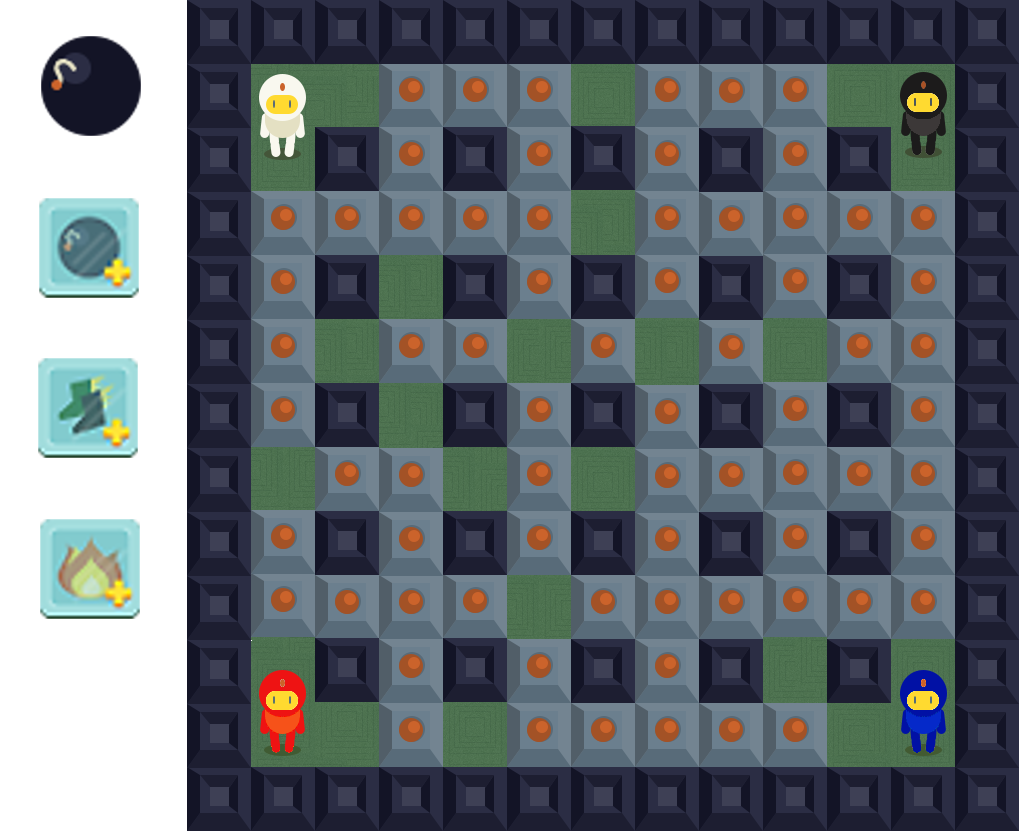
\includegraphics[scale=0.8]{bombermangame.png}
	\end{center}

\end{frame}

%Domain Modell
\begin{frame}[fragile]
  \frametitle{Domain Modell}

    Insert Domain Modell here

\end{frame}

%Systemarchitektur
\begin{frame}{fragile}
  Insert Architektur here
\end{frame}


%Design
\begin{frame}
    Insert here
\end{frame}


%Team Management
\begin{frame}{fragile}
 Insert Team
\end{frame}
%High Risks Tasks
\begin{frame}{fragile}

\end{frame}
%Demo
\plain{Demonstration}

%probleme & Lösungen
\begin{frame}{fragile}
    insert here
\end{frame}

%Statistiken

\begin{frame}{Bar charts}
  
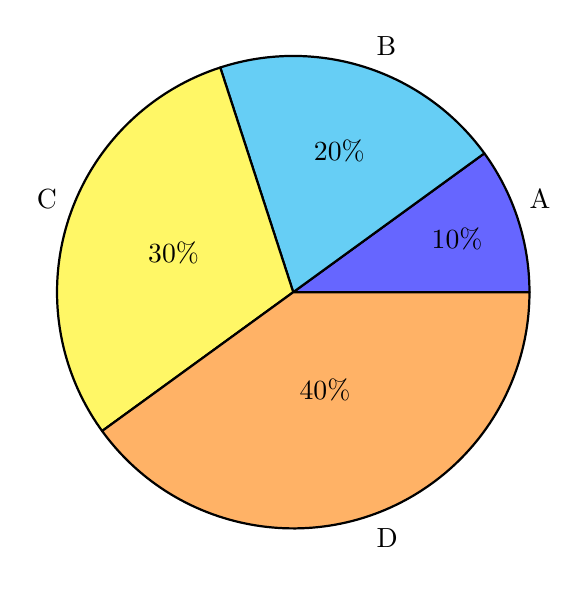
\begin{tikzpicture}
\pie{10/A, 20/B, 30/C, 40/D}
\end{tikzpicture}
\end{frame}
\begin{frame}{Quotes}
  \begin{quote}
    Veni, Vidi, Vici
  \end{quote}
\end{frame}

%Fazit,Lessons learned
\section{Fazit}
\begin{frame}{Summary}
Teamarbeit -> besser im Team arbeiten
Projektmanagement
Viel genauer Anforderungen beschreiben/setzen (z.B.: Git)

\end{frame}

\plain{Fragen?}

\end{document}
